\section{VLAKKE MEETKUNDE} \label{vlakke meetkunde}
\hypertarget{vlakke_meetkunde}{}

\subsection{Hoeken} \label{hoeken}
\hypertarget{hoeken}{}

\begin{minipage}{0.2\linewidth}
\definecolor{qqwuqq}{rgb}{0,0.39,0}
\definecolor{qqqqff}{rgb}{0,0,1}
\begin{tikzpicture}[scale=0.4,line cap=round,line join=round,>=triangle 45,x=1.0cm,y=1.0cm]
\clip(0,0) rectangle (5,5);
\draw [shift={(1,1)},color=qqwuqq,fill=qqwuqq,fill opacity=0.1] (0,0) -- (0:0.55) arc (0:38.66:0.55) -- cycle;
\draw [domain=1.0:5.0] plot(\x,{(--7-0*\x)/7});
\draw [domain=1.0:5.0] plot(\x,{(--1--4*\x)/5});
\begin{scriptsize}
\fill [color=qqqqff] (1,1) circle (1.5pt);
\draw[color=qqqqff] (0.71,0.83) node {$A$};
\draw[color=qqwuqq] (1.95,1.33) node {$\alpha$};
\draw[color=black] (3.9,0.8) node {$a$};
\draw[color=black] (3.4,3.4) node {$b$};
\end{scriptsize}
\end{tikzpicture}
 % todo: andere figuren in document gebruiken hoofdletter voor rechte, kleine letter voor punt..
\end{minipage}
\begin{minipage}{0.8\linewidth}
Een {\bf hoek} $\alpha$ wordt gevormd door twee halfrechten met zelfde beginpunt $A$. De halfrechten $a$ en $b$ worden de {\bf benen} van de hoek genoemd.
\end{minipage}


\subsubsection{Soorten hoeken}
\begin{itemize}
  \item Een {\bf scherpe hoek} is kleiner dan $90\degree$.
  \item Een {\bf rechte hoek} is $90\degree$.
  \item Een {\bf stompe hoek} is groter dan $90\degree$.
  \item Een {\bf gestrekte hoek} is $180\degree$.
  \item Twee hoeken zijn {\bf supplementaire hoeken} als hun som een gestrekte hoek is.
  \item Twee hoeken zijn {\bf complementaire hoeken} als hun som een rechte hoek is.
  \item Twee {\bf aanliggende hoeken} zijn hoeken met een zelfde beginpunt en één been gemeenschappelijk.
  \item Twee aanliggende hoeken zijn {\bf nevenhoeken} als hun som $180\degree$ is.
\end{itemize}

\subsection{Stelling van Thales} \label{thales}
\hypertarget{thales}{}
De lijnstukken ingesneden door evenwijdige rechten op een snijlijn zijn evenredig met de overeenkomende lijnstukken ingesneden op elke andere snijlijn.

\[\ds\Frac{|ab|}{|bc|}=\ds\Frac{|a'b'|}{|b'c'|}\]
%\docLink[tekening]{thales.jpg}{\includegraphics{tekening.gif}}\newline
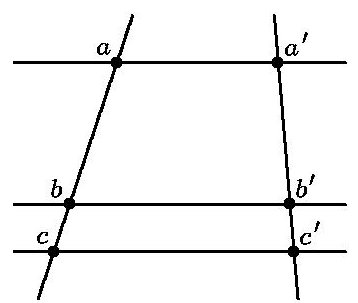
\includegraphics{thales.jpg}
In het bijzonder geldt bij evenwijdige projectie:
De projecties van evenwijdige lijnstukken hebben dezelfde verhouding als de lijnstukken zelf.

\subsection{Driehoeken} \label{driehoeken}
\hypertarget{driehoeken}{}

%\docLink[tekening]{driehoek.jpg}{\includegraphics{tekening.gif}}
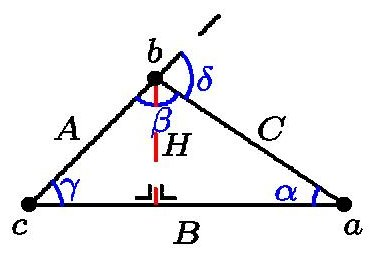
\includegraphics{driehoek.jpg}

\subsubsection{Oppervlakte (O)} \label{oppervlakte driehoek}
\hypertarget{oppervlakte_driehoek}{}
	\[O=\ds\Frac{B\cdot H}{2}\]
	Of ook:\newline\label{alternatief}
	\begin{eqnarray*}
	O &=&\ds\Frac{1}{2}\cdot A\cdot B\cdot \sin\gamma \\
	  &=&\ds\Frac{1}{2}\cdot B\cdot C\cdot \sin\alpha \\
	  &=&\ds\Frac{1}{2}\cdot C\cdot A\cdot \sin\beta \\
	\end{eqnarray*}

\subsubsection{Eigenschappen} \label{eigenschappen}
\hypertarget{eigenschappen}{}
		\begin{itemize}%eign
		\item De {\bf som van de hoeken} van een driehoek is 	$180^{\circ}$.
		\[\alpha+\beta+\gamma=180^{\circ}\]
		\item Een \hypertarget{buitenhoek}{{\bf buitenhoek}} \label{buitenhoek} van een driehoek is gelijk aan de som 		van de niet-aanliggende binnenhoeken.
		\[\delta=\alpha+\gamma\]
		\item In een rechthoekige driehoek geldt de stelling van \hypertarget{pythagoras}{{\bf Pythagoras}}: 		\label{Pythagoras} \[C^2=A^2+B^2\] met $C$ de schuine zijde en $A, B$ de 		rechthoekzijden.
		\end{itemize}%eign

\subsubsection{Merkwaardige lijnen} \label{merkwaardige_lijnen}
\hypertarget{merkwaardige_lijnen}{}
		\begin{itemize}%merkw lijnen
		\item \hypertarget{zwaartelijn}{{\bf Zwaartelijnen $(Z_a, Z_b, Z_c)$}}\label{zwaartelijn}\newline
		De drie zwaartelijnen gaan door \'e\'en punt, het zwaartepunt.\newline\newline
		{\bf Eigenschap v.h. zwaartepunt:}het zwaartepunt verdeelt de zwaartelijnen in twee 		stukken waarvan de lengtes zich verhouden als 2 en 1.
		\[|m_az|=\ds\Frac{1}{2}|za|\]
		%\docLink[tekening]{zwaartelijnen.jpg}{\includegraphics{tekening.gif}}
                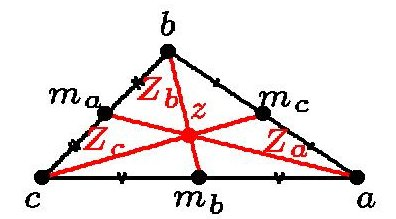
\includegraphics{zwaartelijnen.jpg}
		\item \hypertarget{hoogtelijn}{{\bf Hoogtelijnen $(H_a, H_b, H_c)$}}\label{hoogtelijn}\newline
		De drie hoogtelijnen gaan door \'e\'en punt.\newline
		%\docLink[tekening]{hoogtelijnen.jpg}{\includegraphics{tekening.gif}}
                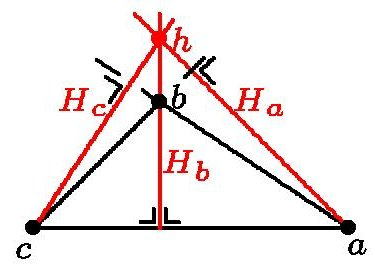
\includegraphics{hoogtelijnen.jpg}
		\item \hypertarget{bissectrice}{{\bf Bissectrices of deellijnen $(D_a, D_b, D_c)$}}\label{bissectrice}\newline
		De drie bissectrices gaan door \'e\'en punt dat bovendien het middelpunt is van de 		ingeschreven cirkel.\newline
		%\docLink[tekening]{bissectrices.jpg}{\includegraphics{tekening.gif}}
                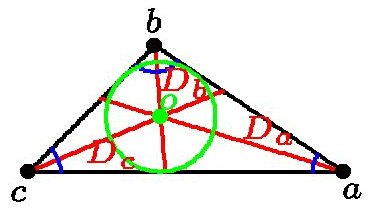
\includegraphics{bissectrices.jpg}
		\item \hypertarget{middelloodlijn}{{\bf Middelloodlijnen $(M_1, M_2, M_3)$}}\label{middelloodlijn}\newline
		De drie middelloodlijnen gaan door \'e\'en punt dat bovendien het middelpunt is van 		de omgeschreven cirkel.\newline
		%\docLink[tekening]{middelloodlijnen.jpg}{\includegraphics{tekening.gif}}
                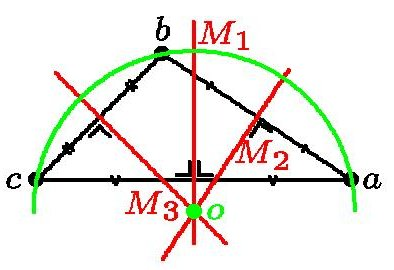
\includegraphics{middelloodlijnen.jpg}
		\end{itemize}%merkw lijnen

\subsubsection{De middenparallel} \label{middenparallel}
\hypertarget{middenparallel}{}
		De {\bf middenparallel} van een driehoek is het lijnstuk dat de middens van twee 		zijden verbindt. Een driehoek heeft er drie. Er geldt bovendien: $|m_1m_2| = 		\ds\Frac{1}{2}|ac|$\newline
		%\docLink[tekening]{middenparallel.jpg}{\includegraphics{tekening.gif}}
                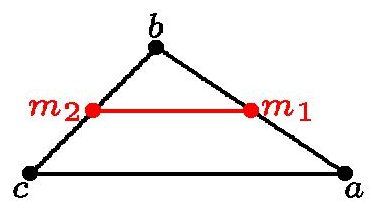
\includegraphics{middenparallel.jpg}

\subsubsection{Congruente driehoeken} \label{congruente_driehoeken}
\hypertarget{congruente_driehoeken}{}
		\begin{itemize}%congruent
		\item \hypertarget{congruente_veelhoeken}{{\bf Definitie congruente veelhoeken:}} \label{congruente_veelhoeken} Congruente veelhoeken 		zijn veelhoeken die door verplaatsing in elkaar kunnen overgaan m.a.w. die elkaar 		volledig kunnen bedekken.
		\item {\bf Gevallen van congruentie bij driehoeken}
			\begin{itemize}%gevallen v. congr.
			\item[*] Twee driehoeken zijn congruent als ze \'e\'en zijde en twee hoeken 			gelijk hebben.
			\item[*] Twee driehoeken zijn congruent als ze twee zijden en de ingesloten 			hoek gelijk hebben.
			\item[*] Twee driehoeken zijn congruent als ze de drie zijden gelijk hebben.
			\end{itemize}%gevallen v. congr.
		\end{itemize}%congruent

\subsubsection{Gelijkvormige driehoeken} \label{gelijkvormige_driehoeken}
\hypertarget{gelijkvormige_driehoeken}{}
		\begin{itemize}%gelijkvormig
		\item {\bf Definitie gelijkvormige veelhoeken:} Gelijkvormige veelhoeken zijn 		veelhoeken die gelijke hoeken hebben en waarvan de overeenkomstige zijden evenredig 		zijn.\newline
		{\bf Gevolg:}\newline\newline
		\begin{tabular}{c}
		$\triangle{abc} \sim \triangle{a'b'c'}$\\
				 $\Updownarrow$ 	\\
            $\ds\Frac{|ab|}{|a'b'|}=\Frac{|bc|}{|b'c'|}=\Frac{|ca|}{|c'a'|}$ \\ 		\end{tabular}		
		\item {\bf Gevallen van gelijkvormigheid bij driehoeken}
			\begin{itemize}%gevallen gelijkv.
			\item[*] Twee driehoeken zijn gelijkvormig als ze twee hoeken gelijk hebben.
			\item[*] Twee driehoeken zijn gelijkvormig als twee zijden van de ene evenredig 			zijn met twee zijden van de andere en de ingesloten hoeken gelijk zijn.
			\item[*] Twee driehoeken zijn gelijkvormig als de drie zijden van de ene 			evenredig zijn met de drie zijden van de andere.
			\item[*] Twee driehoeken zijn gelijkvormig als de zijden van de ene evenwijdig 			lopen met of loodrecht staan op de zijden van de andere.
			\end{itemize}%gevallen gelijkv
		\end{itemize}%gelijkvormig

\subsubsection{Driehoeksongelijkheid} \label{driehoeksongelijkheid}
\hypertarget{driehoeksongelijkheid}{}

%\docLink[tekening]{driehoeksongelijkheid.jpg}{\includegraphics{tekening.gif}}\newline
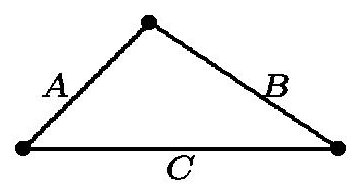
\includegraphics{driehoeksongelijkheid.jpg}
		Zij $A, B$ en $C$ de lengtes van de zijden van een driehoek ($A\:\leq\: B\leq 		C$), dan geldt:
		\[C-B\:\leq \:A\leq B+C\]
		\[C-A\:\leq \:B\leq A+C\]
		\[B-A\:\leq C\:\leq B+A\]

\subsection{Vierhoeken} \label{vierhoeken}
\hypertarget{vierhoeken}{}

\subsubsection{Parallellogram} \label{parallellogram}
\hypertarget{parallellogram}{}
		\begin{itemize}%par
		\item[*]{\bf Definitie:} Een parallellogram is een vierhoek waarvan de 		overstaande zijden evenwijdig zijn.\newline
		%\docLink[tekening]{parallellogram.jpg}{\includegraphics{tekening.gif}}
                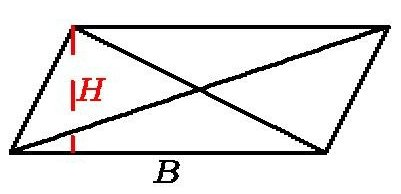
\includegraphics{parallellogram.jpg}
		\item[*]{\bf Oppervlakte (O):} $O = B\cdot H$
		\item[*]{\bf Eigenschap:} De diagonalen snijden elkaar middendoor.
		\item[*]{\bf Speciale gevallen:}
			\begin{itemize}
			\item[$\bullet$]Een {\bf ruit} is een vierhoek met vier gelijke 			zijden.\newline
			{\bf Eigenschap:} De diagonalen staan loodrecht op elkaar en delen de 			hoeken middendoor.
			%\docLink[tekening]{ruit.jpg}{\includegraphics{tekening.gif}}
                        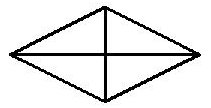
\includegraphics{ruit.jpg}
			\item[$\bullet$]Een {\bf rechthoek} is een vierhoek met vier gelijke 			hoeken.\newline 
			{\bf Eigenschap:} De diagonalen zijn gelijk.\newline
			%\docLink[tekening]{rechthoek.jpg}{\includegraphics{tekening.gif}}
                        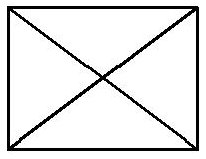
\includegraphics{rechthoek.jpg}
			\item[$\bullet$]Een {\bf vierkant} is een rechthoek met vier gelijke 			zijden.\newline
			%\docLink[tekening]{vierkant.jpg}{\includegraphics{tekening.gif}}
                        
\includegraphics{vierkant.jpg}
			\end{itemize}
		\end{itemize}%par

\subsubsection{Trapezium} \label{trapezium}
\hypertarget{trapezium}{}
		\begin{itemize}%trap 
		\item[*]{\bf Definitie:}
		Een trapezium is een vierhoek met twee evenwijdige zijden.
		\item[*]{\bf Oppervlakte (O):} $O=\ds\Frac{b+B}{2}\cdot H$
		\item[*]{\bf Middenparallel:}$|m_1m_2|=\ds\Frac{b+B}{2}$
		\end{itemize}%trap
		%\docLink[tekening]{trapezium.jpg}{\includegraphics{tekening.gif}}
                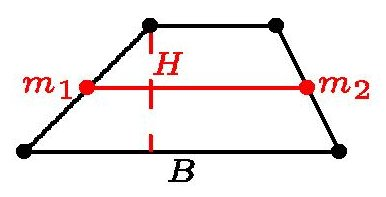
\includegraphics{trapezium.jpg}

\subsection{Veelhoeken} \label{veelhoeken}
\hypertarget{veelhoeken}{}
	\begin{itemize}%veelh
	\item De som van de hoeken van een n-hoek is gelijk aan: $(n-2)180^{\circ}$
	\item Elke hoek van een {\bf regelmatige n-hoek} is gelijk aan: $\ds\Frac{(n-	2)180^{\circ}}{n}$
	\end{itemize}%veelh

\subsection{Cirkels} \label{cirkels}
\hypertarget{cirkels}{}
Zij $r$ de straal van de cirkel.\newline

\subsubsection{Omtrek:} \label{omtrek_cirkel}
\hypertarget{omtrek_cirkel}{}
$2\pi r$ 

\subsubsection{Oppervlakte:}\label{oppervlakte_cirkel}
\hypertarget{oppervlakte_cirkel}{}
$\pi r^2$

\subsubsection{Raaklijn-normaal} \label{raaklijn-normaal}
\hypertarget{raaklijn-normaal}{}
	\begin{itemize}
	\item[*] Een {\bf raaklijn} aan een cirkel is een rechte die juist \'e\'en punt gemeen 	heeft met de cirkel.
	\item[*] Een raaklijn aan een cirkel staat loodrecht op de straal naar het raakpunt.
	\item[*] De {\bf normaal} in een punt op de cirkel is de loodlijn in dit punt op de 	raaklijn.
	\end{itemize}

\subsubsection{Boog-koorde} \label{boog-koorde}
\hypertarget{boog-koorde}{}
	\begin{itemize}
	\item[*]Een {\bf boog} is een deel van de cirkelomtrek.
	\item[*]{\bf Lengte van een \hypertarget{cirkelboog}{cirkelboog}:} $\alpha r$\label{cirkelboog}\newline
	\item[*]Een {\bf koorde} is een lijnstuk dat de eindpunten van een boog verbindt.
	\end{itemize}
	%\docLink[tekening]{cirkel.jpg}{\includegraphics{tekening.gif}}
        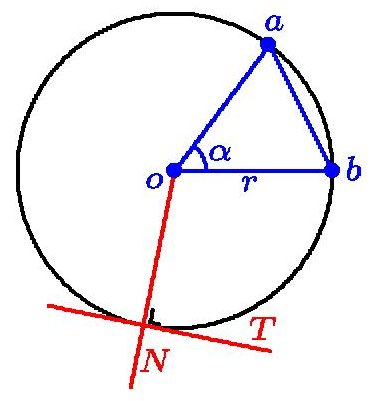
\includegraphics{cirkel.jpg}

\subsubsection{Middelpuntshoek-omtrekshoek} \label{middelpunts-omtrekshoek}
\hypertarget{middelpunts-omtrekshoek}{}
	\begin{itemize}
	\item[*] Een {\bf omtrekshoek} meet de {\bf helft} van de middelpuntshoek op dezelfde 	boog.
	\item[*] Omtrekshoeken die op eenzelfde boog staan, zijn gelijk.
	\end{itemize}
	%\docLink[tekening]{omtrekshoek.jpg}{\includegraphics{tekening.gif}}
        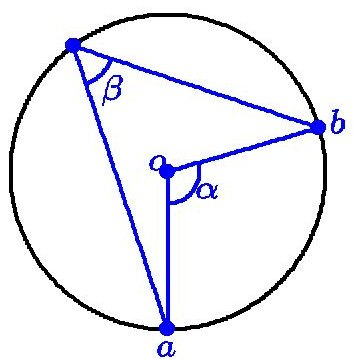
\includegraphics{omtrekshoek.jpg}

\subsubsection{Binnen- en buitenomtrekshoek} \label{binnen-buitenomtrekshoek} 
\hypertarget{binnen-buitenomtrekshoek}{}
	\begin{itemize}
	\item[*] Een {\bf binnenomtrekshoek} heeft hetzelfde maatgetal als de halve {\bf som} van 	de boog binnen de hoek en de boog binnen de overstaande hoek.
	\[\alpha=\ds\Frac{1}{2}(\stackrel{\frown}{ab}+\stackrel{\frown}{cd})\]
	%\docLink[tekening]{binnenomtrk.jpg}{\includegraphics{tekening.gif}}
        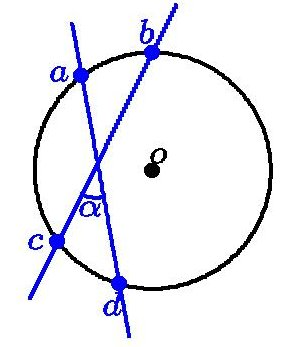
\includegraphics{binnenomtrk.jpg}
	\item[*] Een {\bf buitenomtrekshoek} heeft hetzelfde maatgetal als het halve {\bf 	verschil} van de bogen binnen de hoek. 
	\[\alpha=\ds\Frac{1}{2}(\stackrel{\frown}{ab}-\stackrel{\frown}{cd})\]
	%\docLink[tekening]{buitenomtrk.jpg}{\includegraphics{tekening.gif}}
        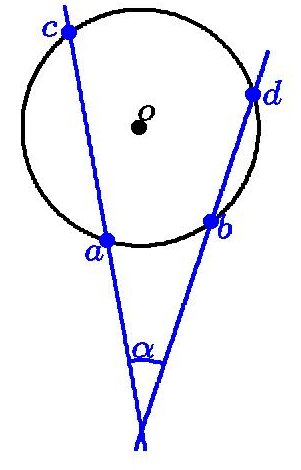
\includegraphics{buitenomtrk.jpg}
	\end{itemize}

\subsubsection{Sector-segment} \label{sector-segment}
\hypertarget{sector-segment}{}
	\begin{itemize}
	\item[*]Een {\bf cirkelsegment} is de figuur gevormd door een boog en zijn koorde.\newline
	%\docLink[tekening]{segment.jpg}{\includegraphics{tekening.gif}}
        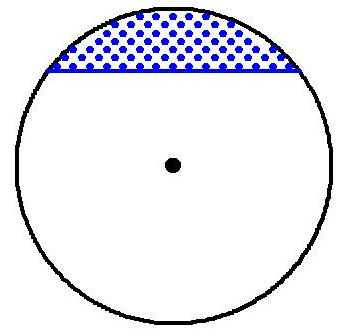
\includegraphics{segment.jpg}
	\item[*]Een \hypertarget{sector}{{\bf cirkelsector}} is de figuur gevormd door een boog en de stralen naar zijn eindpunten.\label{sector}\newline
	%\docLink[tekening]{sector.jpg}{\includegraphics{tekening.gif}}
        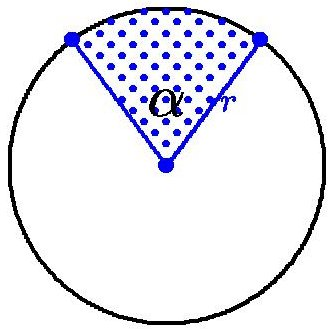
\includegraphics{sector.jpg}
	\item[*] {\bf Oppervlakte van een cirkelsector:} $\ds\Frac{1}{2}\alpha r^2$
	\end{itemize}

\subsubsection{Macht van een punt t.o.v. de cirkel} \label{macht_punt-cirkel}
\hypertarget{macht_punt-cirkel}{}
	Het product van de afstanden van een punt $p$ tot de snijpunten van een veranderlijke 	rechte door $p$ met de cirkel, is constant; die constante noemen we de {\bf macht van 	het punt tot de cirkel}.
	\[|pa|\cdot|pb|=|pc|\cdot|pd|\]
	%\docLink[tekening]{macht.jpg}{\includegraphics{tekening.gif}}
        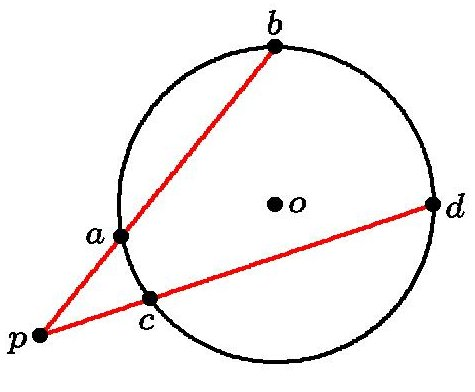
\includegraphics{macht.jpg}

\subsubsection{Koordenvierhoek} \label{koordenvierhoek}
\hypertarget{koordenvierhoek}{}
	\begin{itemize}
	\item[*]Een {\bf koordenvierhoek} is een vierhoek ingeschreven in een cirkel.
	\item[*]In een koordenvierhoek zijn de overstaande hoeken $\alpha$ en $\beta$ elkaars 	supplement.
	\end{itemize}
	%\docLink[tekening]{koordenvierhoek.jpg}{\includegraphics{tekening.gif}}
        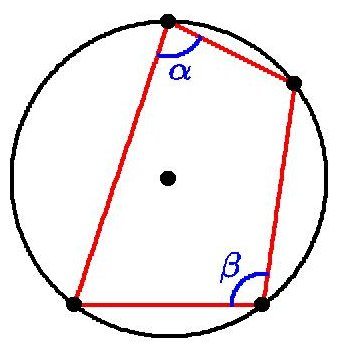
\includegraphics{koordenvierhoek.jpg}

\subsection{Analytische meetkunde} \label{analytische_meetkunde}
\hypertarget{analytische_meetkunde}{}

\subsubsection{Afstand tussen twee punten} \label{afstand_twee_punten}
\hypertarget{afstand_twee_punten}{}
Zij $p(x_1, y_1)$ en $q(x_2, y_2)$ twee punten dan geldt:\newline
\[d(p, q)=|pq|=\sqrt{(x_2-x_1)^2+(y_2-y_1)^2}\]

\subsubsection{Midden van een lijnstuk} \label{midden_lijnstuk}
\hypertarget{midden_lijnstuk}{}
Zij $a(x_1, y_1)$ en $b(x_2, y_2)$ twee punten in het vlak, dan is de co\"ordinaat van het midden $(m)$ van het lijnstuk $[ab]$:
\[co(m)=\left(\ds\Frac{x_1+x_2}{2}, \ds\Frac{y_1+y_2}{2}\right)\]

\subsubsection{Afstand van een punt tot een rechte} \label{afstand_punt-rechte}
\hypertarget{afstand_punt-rechte}{}
Zij $A\:\leftrightarrow\:ax+by+c=0$ een rechte en $p(x_1, x_2)$ een punt, dan geldt:\newline
\[d(p, A)=\ds\Frac{|ax_1+by_1+c|}{\sqrt{a^2+b^2}}\]
De \hypertarget{normaalvergelijking}{{\bf normaalvergelijking}} van een rechte $L\,\leftrightarrow\,ax +by+c=0$ is:\label{normaalvergelijking}
\[\ds\Frac{ax+by+c}{\sqrt{a^2 + b^2}}=0\]

\subsubsection{Loodrechte stand - evenwijdigheid} \label{loodrecht-evenwijdig}
\hypertarget{loodrecht-evenwijdig}{}
\begin{itemize}
\item[*]Twee rechten met respectieve richtingsco\"effici\"enten $m_1$ en $m_2$ staan {\bf loodrecht} op elkaar a.s.a $m_1m_2=-1$.
\item[*]Twee rechten met respectieve richtingsco\"effici\"enten $m_1$ en $m_2$ zijn {\bf evenwijdig} a.s.a. $m_1=m_2$.
\end{itemize}

\subsubsection{De vergelijking van de cirkel} \label{vergelijking_cirkel}
\hypertarget{vergelijking_cirkel}{}
Zij $m(x_1,y_1)$ het middelpunt en $r$ de straal van de cirkel, dan is de (middelpunts)vergelijking:
\[C(m, r)\:\leftrightarrow\:(x-x_1)^2+(y-y_1)^2=r^2\]

\subsection{Vectoren} \label{vectoren}
\hypertarget{vectoren}{}

\subsubsection{Definitie:} \label{definitie}
\hypertarget{definitie}{}
{\bf Vector $\vec{ab}$} is de verzameling van alle lijnstukken die dezelfde lengte, richting en 
zin hebben als het geori\"enteerde lijnstuk $\vec{ab}$.\newline
Grafisch wordt $\vec{ab}$ voorgesteld door \'e\'en representant van die verzameling.\newline
%\docLink[tekening]{vectoren1.jpg}{\includegraphics{tekening.gif}}\newline
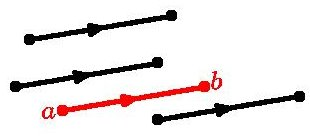
\includegraphics{vectoren1.jpg}
Met {\bf plaatsvector} $\vec{p}$ wordt vector $\vec{op}$ bedoeld, met $o$ de oorsprong van het vlak.\newline
%\docLink[tekening]{vectoren2.jpg}{\includegraphics{tekening.gif}}
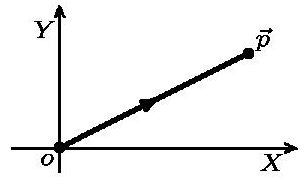
\includegraphics{vectoren2.jpg}

\subsubsection{Co\"ordinaat van een vector (componentenkoppel)} \label{coordinaten}
\hypertarget{coordinaten}{}
Bij plaatsvectoren geldt: co$(\vec{p})=co(p)=(x_1, x_2)$\newline
De co\"ordinaat van $\vec{ab}$ is dezelfde als die van zijn plaatsvector.\newline
%\docLink[tekening]{vectoren3.jpg}{\includegraphics{tekening.gif}}
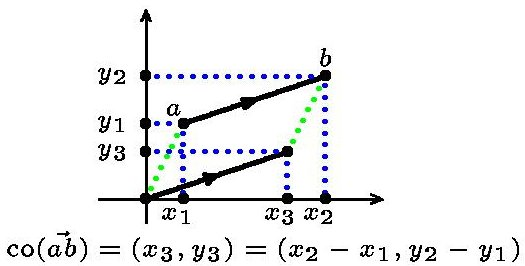
\includegraphics{vectoren3.jpg}

\subsubsection{Optellen van vectoren} \label{optellen_vectoren}
\hypertarget{optellen_vectoren}{}
Voor het optellen van vectoren geldt de regel van het parallellogram.\newline
%\docLink[tekening]{vectoren4.jpg}{\includegraphics{tekening.gif}}\newline
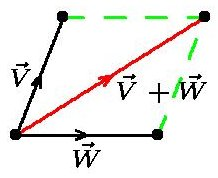
\includegraphics{vectoren4.jpg}
Met co\"ordinaten: als co$(\vec{V})=(x_1, y_1)$ en co($\vec{W})=(x_2, y_2)$ dan is:
\[co(\vec{V}+\vec{W})=(x_1 +x_2, y_1+y_2)\]

\subsubsection{Scalaire vermenigvuldiging} \label{scalaire_vermenigv}
\hypertarget{scalaire_vermenigv}{}
Het $r$-voud van een vector $\vec{V}$ is een vector met lengte $|r|$ maal de lengte van $\vec{V}$, richting dezelfde als die van $\vec{V}$ en zin dezelfde als die van $\vec{V}$ (r>0) of tegengesteld aan die van $\vec{V}$ (r<0).\newline
Met co\"ordinaten: als co$(\vec{V})=(x_1, y_1)$, dan is:
\[co(r\vec{V})=(rx_1, ry_1)\]

\subsubsection{Norm van een vector} \label{norm_vector}
\hypertarget{norm_vector}{}
De norm van een vector: $\|\vec{ab}\|$ is de afstand d$(a, b)$.\newline
Met co\"ordinaten: als co$(\vec{V})=(x_1, y_1)$ dan is:
\[\|\vec{V}\| = \sqrt{x_1^2 + y_1^2}\]

\subsubsection{Ongelijkheid van Minkowski} \label{minkowski}
\hypertarget{minkowski}{}
\[\|\vec{V}+\vec{W}\|\, \leq\, \|\vec{V}\| + \|\vec{W}\|\]

\subsubsection{Hoek tussen twee vectoren} \label{hoek_vectoren}
\hypertarget{hoek_vectoren}{}

Als $\vec{U}$ en $\vec{V}$ verschillend zijn van $\vec{0}$, co($\vec{U})=(x_1, y_1)$ en co($\vec{V})=(x_2, y_2)$ en $\varphi$ de hoek tussen beide vectoren, dan is: 
\[cos(\varphi)=\ds\Frac{x_1x_2+y_1y_2}{\sqrt{x_1^2+y_1^2}\cdot\sqrt{x_2^2+y_2^2}}\]

\subsubsection{Scalair product van twee vectoren} \label{scalair_product_vectoren}
\hypertarget{scalair_product_vectoren}{}
Als $\vec{U}$ en $\vec{V}$ verschillend zijn van $\vec{0}$ en $\varphi$ de hoek is tussen beide vectoren, dan is het scalair product:
\[\vec{U}\cdot \vec{V} = \|\vec{U}\|\cdot\|\vec{V}\|\cdot \mbox{cos}(\varphi)\]
Met co\"ordinaten: 
\[\vec{U}\cdot\vec{V}=x_1x_2+y_1y_2\]

\subsubsection{Orthogonaliteit van vectoren:} \label{orthogonaliteit_vectoren}
\hypertarget{orthogonaliteit_vectoren}{}
Twee vectoren $\vec{U}$ en $\vec{V}$ zijn orthogonaal als $\vec{U}\cdot \vec{V}=0$.


% Dit werk is gelicenseerd onder een Creative Commons
% Naamsvermelding-GelijkDelen 3.0 Unported.
% Bezoek http://creativecommons.org/licenses/by-sa/3.0/ om een kopie te zien 
% van de licentie of stuur een brief naar Creative Commons, 444 Castro Street, 
% Suite 900, Mountain View, California, 94041, USA.
